% file: example.tex
%
% Use:
% 	$ pdflatex -shell-escape <filename.tex>
% to generate a png image.

\documentclass[11pt,tikz,border=1,convert={outfile=\jobname.png}]{standalone}
\usetikzlibrary{calc,positioning,arrows.meta,shadows}

\begin{document}
  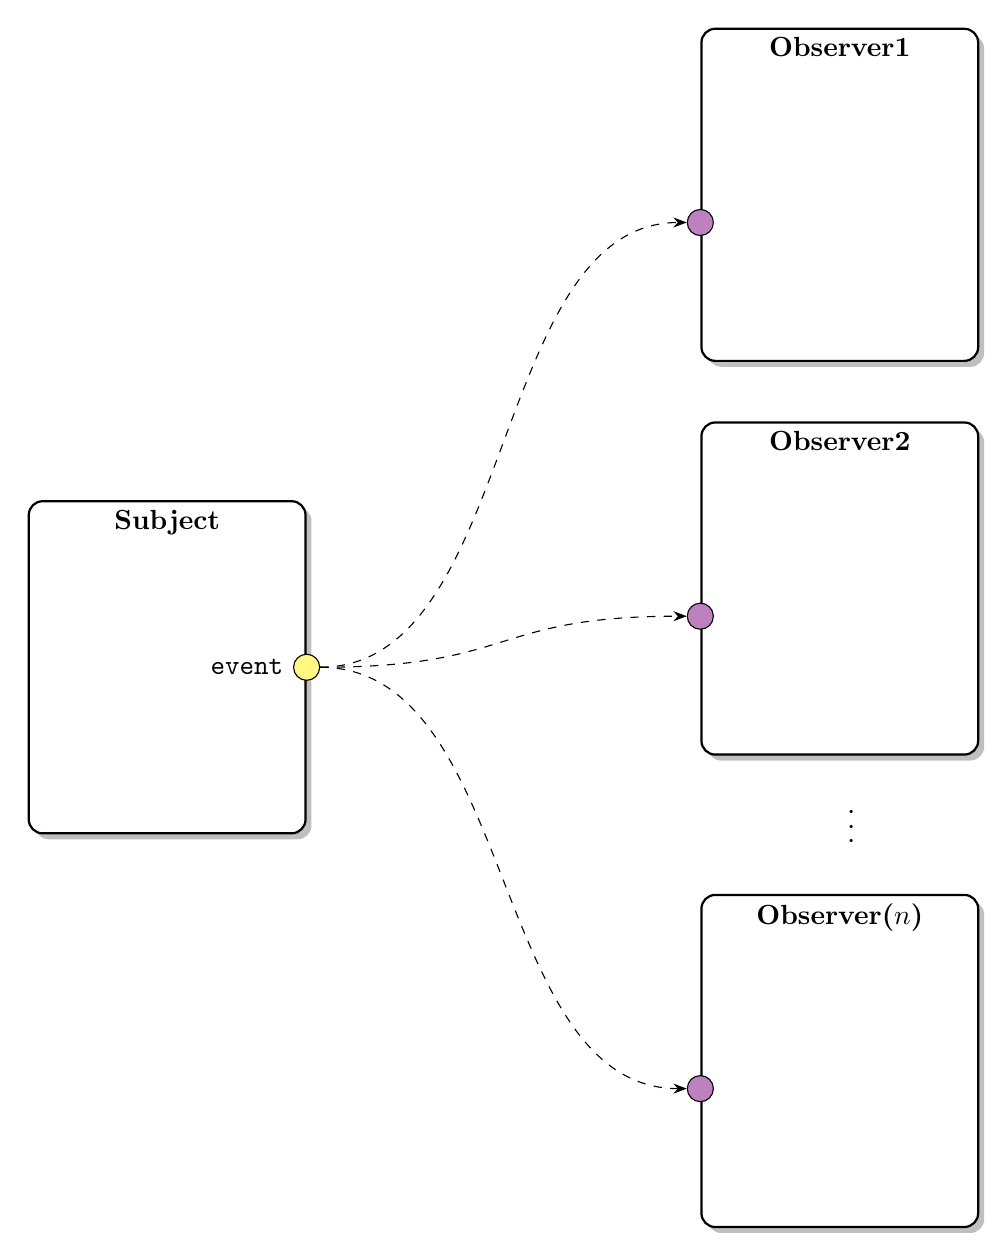
\begin{tikzpicture}[
    object/.style={thick,fill=white,rectangle,rounded corners=5pt,draw,minimum width=100pt,minimum height=120pt,drop shadow},
    token/.style={circle,draw,fill=yellow!50,minimum size=6pt},
    binding/.style={circle,draw,fill=violet!50,minimum size=6pt}
    ]

  \node(subject) [object] {};
  \node(subjectName) [below] at (subject.north) {\bf Subject};
  \node(event1) [token] at (subject.east) {};

  \node(observer1) [right=5cm of subject,yshift=6cm,object] {};
  \node(observer1Name) [below] at (observer1.north) {\bf Observer1};
  \node(method1) [binding,yshift=-10pt] at (observer1.west) {};

  \node(observer2) [right=5cm of subject,yshift=1cm,object] {};
  \node(observer2Name) [below] at (observer2.north) {\bf Observer2};
  \node(method2) [binding,yshift=-10pt] at (observer2.west) {};

  \node(observer3) [right=5cm of subject,yshift=-5cm,object] {};
  \node(observer3Name) [below] at (observer3.north) {\bf Observer($n$)};
  \node(method3) [binding,yshift=-10pt] at (observer3.west) {};

  \node [below,rotate=90,xshift=-9mm] at (observer2.south) {\large $\ldots$};

  \coordinate(a) at ($(event1.east)+(25mm,0)$);
  \coordinate(b) at ($(method1.west)-(25mm,0)$);
  \coordinate(c) at ($(method2.west)-(25mm,0)$);
  \coordinate(d) at ($(method3.west)-(25mm,0)$);

  \draw[->,dashed,-{Stealth}] (event1) .. controls (a) and (b) .. (method1);
  \draw[->,dashed,-{Stealth}] (event1) .. controls (a) and (c) .. (method2);
  \draw[->,dashed,-{Stealth}] (event1) .. controls (a) and (d) .. (method3);

  \node [left] at (event1.west) {\ttfamily event};

  \end{tikzpicture}
\end{document}
